\chapter{Methodology} % Main chapter title

\section{Complex networks}
The complex system has several properties. It consists of many components such as units or individuals who interact with each other. The properties of the complex system can not be predicted from the behaviour of one individual. In such systems, without any central force, collective behaviour can emerge. In societies, people's interactions lead to civilisation, economy, formation of social groups or even traffic on the roads. In the animal, populations are present at different levels of the organisation, as in ants and bees colonies or the school of the fishies showing flocking patterns. \cite{boccaletti2006complex}
%latorobook 

The research in complex systems focuses on the structure of the interactions between units. Knowing how branches of the system are connected, we can determine the emergence of the collective behaviour of the system. We can construct networks with neurons and synapses, representing their connections. The structure of the brain network and its properties are fundamental for brain functioning, and neurons in the same brain area are closely connected. Similarly, we can represent the communication between people. The structure of these interactions gives us insights, for example, how information propagates through the system. The presence of people with many connections can lead to faster information flow. 

Despite the differences between complex systems, they can be studied using complex networks; with sets of nodes and edges. Elements in the system are nodes, while interactions between them are given as edges. This approximation allows us to treat equally social (graph of actors), biological (network of proteins) or even technological systems (internet, traffic). In recent years, complex network theory has application in different fields, and the availability of big data incurs its development. \\
%Analyzing and Modeling Real-World Phenomena with Complex Networks: A Survey of Applications
%Characterization of Complex Networks: A Survey of measurements

The complex network theory originates from the graph theory in mathematics. These days, the graph and network are used as equivalent terms. The first mathematical problem solved using graph theory was $Konigsberg$ problem of seven bridges. The city $Konigsberg$ had seven bridges connecting the city's parts across the river and the island in the middle. The question was, is it possible to find a walk that crosses all seven bridges only once. Representing the problem as a graph, Euler managed to simplify the problem; the parts of the land are represented as nodes while bridges between them are links. Crossing each bridge only once is possible if each part of the land has an even number of connections. Thus, it was not possible in this case, as each piece of land had an odd number of bridge connections, see Fig. \ref{fig:Krgraph}.

\begin{figure}[h!]
	\centering
	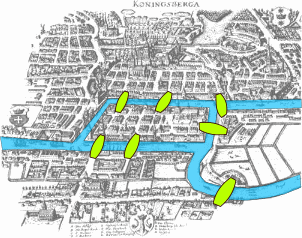
\includegraphics[width=0.3\linewidth]{Figures/Konigsberg_bridges.png} \hspace{2cm}
	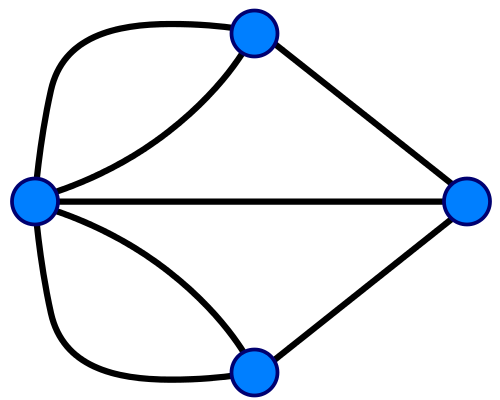
\includegraphics[width=0.3\linewidth]{Figures/Konigsberg_graph.png}
	\caption{The Kronigsber problem of seven bridges.}
	\label{fig:Krgraph}
\end{figure}

\section{Types of networks}

%The seven bridges problem in Fig. \ref{fig:Krgraph} is represented with the \textbf{simple network} structure. 
The graph or network $G$ is defined as $G=(V, E)$, where $V$ is a set of nodes (vertices), and $E$ is a set of edges. The edge is pair of nodes $e_{ij} = (i, j), $ and $i,j\in E$. The graph structure has undirected edges meaning that edges are symmetric: $(i, j)$ implies $(j, i)$. Edges are also unweighted, meaning that all edges are equally important. The specific properties of the nodes are also neglected in this representation. The \textbf{adjacency matrix} ${A} = N \times N$ has value $1$ if there is connection between two nodes, otherwise it is $0$ \cite{boccaletti2006}\\

For example, if we consider unweighted, undirected network, with only 3 nodes and two connections, adjacency matrix is:


\begin{equation}
A = \begin{bmatrix}
0 & 1 & 1\\
1 & 0 & 0 \\
1 & 0 & 0 \\
\end{bmatrix}
\end{equation}

The self loops usually are not considered, meaning that $A_{ii}=0$. 
%The complex system can be represented by complex network $G=(V, E)$, where the elements of system (atoms, proteins, people) map to set of $N$ nodes $V=\{1, 2, ...,N\}$. The interactions between elements map to $L$ links between nodes, $E = \{ e_1, e_2... e_L\}$. The \textbf{adjacency matrix} ${A} = N \times N$ has value $1$ if there is connection between two nodes, otherwise it is $0$ \cite{boccaletti2006}.

Other equivalent way of representing graph is as edge list. Instead of having adjacency matrix, graph is described with the list of links that are in graph. The graph is then pair of $N, g$, where N is set of nodes, and $g$ is collection of links, listed as subset of $N$ of size 2. So the network is written as $g = \{ \{1,2\}, \{2,3\}\}$.

Sometimes it is essential to include specific properties of the system in the network representation, which can help create more realistic models. The additional properties can be added on the edge, node or network level. \\

\begin{figure}[h!]
	\centering
	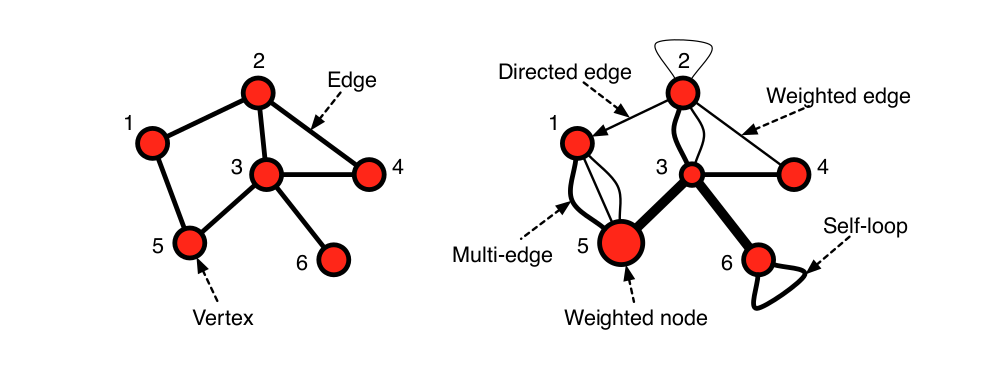
\includegraphics[width=1\linewidth]{figures/methodology/graph1.png} 
	\caption{Graph types}
	\label{fig:gt1}
\end{figure}

In a \textbf{directed network}, edges have broken symmetry. The interaction from node $i$ to node $j$ does not need to have the same property as the interaction from node $j$ to node $i$. A typical example is WWW, where webpages are nodes, and hyperlinks are directed edges. In biological networks, gene regulation and neural activation can be given as directed networks. \\ %clasuet networks

\begin{figure}[h!]
	\centering
	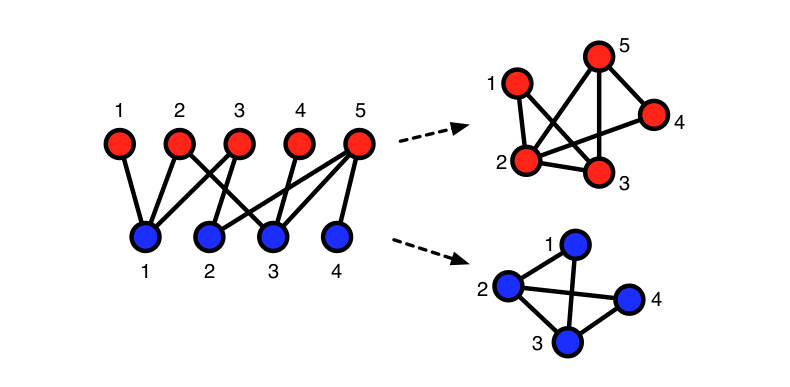
\includegraphics[width=0.8\linewidth]{figures/methodology/graph2.png} 
	\caption{Graph types}
	\label{fig:gt2}
\end{figure}

The frequency of interaction between nodes is emphasised if edges are associated with different scalar values; networks are \textbf{weighted}. The edges may be signed, representing activation in the biological system or trust and distrust in the social system. In general, edges can be associated with any categorical variable. If attribute describes the time when an interaction between nodes happened; network is called \textbf{temporal}. Finally, \textbf{multigraph} allows the presence of multiply edges between two nodes. For the network between cities, edges may be different driving paths between them. In neuron cells, multiply synapses are represented as distinct edges. \\

A \textbf{bipartite network} has two partitions, $U$ and $V$. The nodes in the same partition are not connected while links exist only between nodes of a different kind. In general, we can define k-bipartite graph. The set of nodes $V$ has $k$ distinct classes of nodes. When $k=2$ the network is bipartite.  Bipartite networks represent the membership of people or items in groups. For example, we can define the network of actors as a bipartite graph. In one partition are actors and in other movies. There are no edges between actors or movies, but the actor is connected to the film if it plays in that movie. Another example is a recommender network, such as a network of people and items they like. 

The equivalent representation of bipartite network is incidence matrix $B$. If $n$ is number of people and $g$ number of groups, this matrix is $g x n$, having elements $B_{ij}$ 1 if persoon i belongs to group j. 

Even bipartite networks give realistic representation of the system, there is often need to analyze the single type of nodes.  From a bipartite network, we can generate two projections. The first one connects nodes partition $V$ if they point to node $u$. Similarly, we can project the network on U partition, connecting $u$ nodes. The one mode projection between actors and movies onto actors is undirected network of actor collaborations. Actors are connected if they appear in the same movie. We can also create one-mode projection onto movies, where two movies are connected if they share the same actor.  

The projections are useful in some manner, but they also lose some important information, for example how many groups nodes share in common. This information can be propagated adding the weight to the edges, equal to the number of common groups.

The product $B_{ki}$ and $B_{kj}$ is 1 if $i$ and $j$ belong to the same group $k$. Thus the total number of groups to which nodes $i$ and $j$ belong is $P_{ij} = \sum_{k=1}^g B_{ki}B_{kj} = \sum_{k=1}^g B_{ik}^TB_{kj}$. The matrix $P$ is matrix of one-mode projection. The diagonal elements are non-zero, and represent the number of groups node $i$ belongs to.  To derive the weighted adjacency matrix, the diagonal elements are set to 0. The adjacency matrix of unweighted projection, each non-zero element needs to be replaced with $1$. 

The important consequence of the one-mode projection is the construction of the cliques; subgraph in which every pair of nodes is connected. Every node that is being projected is represented as a clique of size, because all pairs of its neighbours are exactly distance two away from each other. All actors in the movie will be joined in a clique in the one-mode actor projection. %ovo preformulisati

Another consequence of the one-mode projection is that one mode projection may originate from different bipartite networks. Meaning that projection is not one-to-one; no bijection. It is surjective operation, meaning hat any projected network $P$ has at least one bipartite network such that the projection of B results in P. \\ %ovo preformulisati

\begin{figure}[h!]
	\centering
	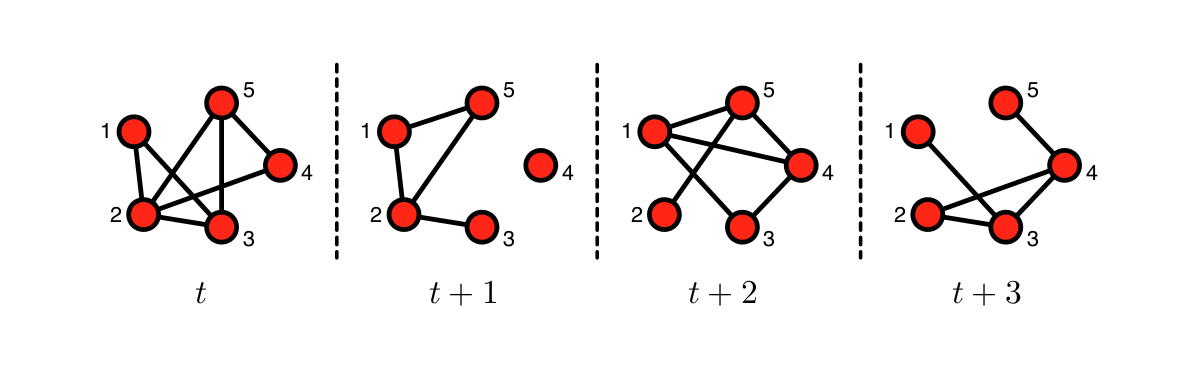
\includegraphics[width=1\linewidth]{figures/methodology/graph4.png} 
	\caption{Graph types}
	\label{fig:gt3}
\end{figure}

In \textbf{temporal networks} nodes and edges evolve. Many real networks are not static, networks grow over time, and edges and nodes may emerge or disappear. Also, some edges may be active at regular intervals, reflecting the circadian rhythms of the nodes. In citation networks, new nodes (paper) join the network, creating links with cited papers. 

Let consider the temporal network with $N$ nodes, over time interval $t_{max}$. The event representation consists in viewing the temporal networks as a collection of time-stamped edges. In this representation, each edge $(i, j)$ is defined as$(i, j, t, \Delta t)$, where $t$ is the time of the event and $\Delta t$ its duration. In a temporal network, the same link can appear multiple times, and the duration of the event may vary. An example of an event temporal network may be phone-calls networks, where a call between two persons $i$ and $j$ started at time $t$ and ended at $t + \Delta t$. 

A temporal network can be represented as sequence of networks $G= G(1), ... G(t_{max})$, where $t_{max}$ is number of networks. While in the event-based representation, time can be both discrete and continuous, in the snapshot representation, time is only discrete. The temporal network is seen as a structure that evolves in time, and at each timestamp, we can analyse the system's macroscopic properties. We need to specify time windows for coarse-grain event-based representation of the temporal information in the data. If we use uniformly time window of length $w$ then the events occurring in $0 \leq t < w$ enter snapshot G(1), those occurring in $w \leq t < 2w$ enter G(2) and so forth. We can not recover the original data points from the snapshot representation, and more information loss is present with a larger time window. If the time window is $w=t_{max}$, there is only one snapshot, temporal data are no more available, and the network is static. \\

\begin{figure}[h!]
	\centering
	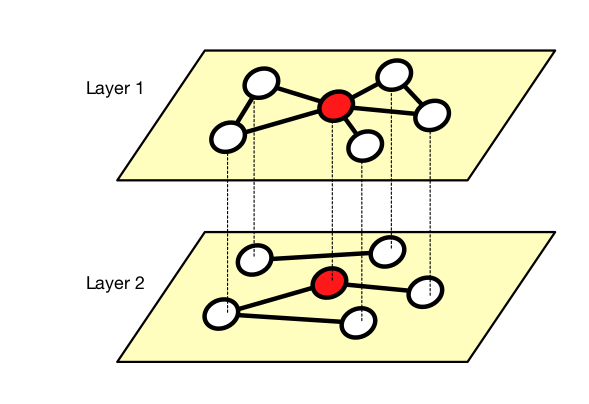
\includegraphics[width=0.5\linewidth]{figures/methodology/graph5.png} 
	\caption{Graph types}
	\label{fig:gt5}
\end{figure}

A network in which edges are marked by which "layer" they exist in is called a multiplex or multilayer network. These networks are used to represent a system in which there are multiple types of interactions, and we store the connectivity of each kind in a different "layer" of the multiplex network. A temporal network is a special kind of multiplex network, where these layers form a temporal (ordered) sequence. Crucially, there can dynamics on each vertex that govern which layer some kind of interaction occurs on, so multiplex networks are not merely a special kind of graph in which different colors or layer numbers annotate edges. %clauset preformulisati

Spatial networks are a special kind of node-annotated network, in which the annotations represent the node's location in some d-dimensional space. This graph property is most common in transportation networks, e.g., as road and city networks, airport transportation networks, oil and gas distribution networks, shipping networks, etc., but can also appear in social networks. Planar graphs are a special case of spatial networks in which the nodes are embedded on a 2-dimensional surface and edges do not cross. %clauset preformulisati

Hypergraphs are another type of network, in which edges denote the interaction of more than two vertices, e.g, E in V × V × V . Scientific collaboration graphs can be represented as a hypergraph, in which each "edge" is the set of coauthors on a scientific article. However, collaboration networks are more commonly represented as bipartite graphs, in which scientists and papers form two sets of vertices, and scientist-nodes are connected to all the paper-nodes on which they are authors. %clauset to do

%The canonical network form is an undirected graph, where two nodes are either connected or not. This applies to situations where two nodes are either in a relationship with each other or not, but it cannot be that one is related to the second without the second being related to the …rst. This is generally true of many social and/or economic relationships, such as partnerships, friendships, alliances, acquaintances, etc. This sort of network will be central to most of the chapters that follow. However, there are other situations that we will examine that are better modeled as directed networks, where one node may be connected to a second without the second being connected to the …rst. For instance, a network that keeps track of which authors cite which other authors, or which web pages have links to which others would naturally take the form  of a directed graph.

\section{The structure of complex networks}

\subsection{Paths and cycles}

As network is connected structure, the nodes may be influenced also by distant nodes, and the information might spread through the links of a network. Analyzing the paths of the network is important task.   

A path of the network between two nodes $i$ and $j$ is a sequence of links, $i_1i_2,..,i_k$ such $i_ki_{k+1} \in g$ that $i_1=i$ and $i_k=j$, each node in the sequence is distinct. 
The path is walk, if nodes in the sequence are not distinct, so walk can visit one node more than once. The cycle is walk that starts and ends at the same node, while other nodes are distinct. 

Note that, if we use adjacency matrix representation where $A_{ii}=0$, then $A^2$ tells us how many walks of length 2 exist between any two nodes.

Network is connected if every two nodes in the network are connected by some path. So the network is connected id for every node $i \in N$ and node $j \in N$ exists a path between them. 

A component of the network are distinct maximal connected subgraphs of a network. In the example there are 4 components. Note that in this definition of the component isolated node is also component. In directed network, set of nodes that are reachable from each other is a strongly connected component, while a set of nodes where either i is reachable from j or j is reachable from i is weakly connected component.

There are a few particular network structures that are commonly referred to.
A tree is a connected network that has no cycles.
A forest is a network such that each component is a tree. Thus any network that
has no cycles is a forest, as in the example pictured in Figure 2.1.6.
A particularly prominent forest network is a star. A star is a network such that
there exists some node i such that every link in the network involves node i. In this
case i is referred to as the center of the star.
There are a few facts about trees that are easy to derive (see Exercise 2.2) and
worth mentioning.
A connected network is a tree if and only if it has n
1 links.
A tree has at least two leaves, where leaves are nodes that have exactly one link.
In a tree, there is a unique path between any two nodes.
The complete network is one where all possible links are present, so one where
where g ij = 1 for all i 6 = j.

A circle (also known as a cycle-graph) is a network that has a single cycle and such
that each node in the network has exactly two neighbors.
In the case of directed networks, there can be many di¤erent stars involving the
same set of nodes and having the same center, depending on which directed links are
present between any two linked nodes. On occasion, it will be useful to distinguish
between these.

Eulerian tours and Hamiltonian cycles

A walk is said to be closed if it starts and ends at the same node. It is clear that in
order to have a closed walk that involves every link of a network exactly once it must
be that each node in the network has an even degree. 39 This follows since each time a
node is “entered” by one link on the walk it must be “exited”by a di¤erent link, and
each time the node is visited, it must be by a link that has not appeared previously on
the walk. Euler’s [?] simple but remarkable theorem is that this condition is necessary
and su¢ cient for there to exist such a closed walk.

A connected network g has a closed walk that involves each link ex-
actly once if and only if the degree of each node is even.


One can ask a related question for nodes rather than links: when is it possible to
…nd a closed walk that involves each node in the network exactly once? Such a closed
walk must be a cycle, and is referred to as a Hamilton Cycle or a Hamiltonian. A
related question is whether there exists a “Hamilton path”that hits each node exactly
once. Clearly a network that has a Hamilton cycle has a Hamilton path, while the
converse is not true (consider a line).
Discovering whether or not a network has a Hamilton cycle is a much more chal-
lenging question than whether it has a Euler tour; and this has been an active area
of research in graph theory for some time. It has direct applications to the “traveling
salesman problem,”where a salesman must visit each city on a trip exactly once, cities
are nodes on a network, and the path must follow the links.
The seminal theorem on Hamilton cycles is due to Dirac [?]. Stronger theorems
have since been developed, as we shall shortly see, but it is worth stating on its own,
as it has an intuitive proof that helps one see the paths to proving some of the later. 


\subsection{community structure}

Thus the ability to find groups or clusters in a network can be a useful tool for revealing structure and organization within networks at a scale larger than that of a single node or a
few nodes. The occurrence of groups or communities is not limited to social networks.
Clusters of nodes in a web network, for instance, might indicate groups of
related web pages. Clusters of nodes in a metabolic network might indicate
functional units within the network. The ability to find groups also has another practical application: it allows
us to take a large network and break it apart into smaller subsets that can be
studied separately. The network in Fig. 14.1 is quite small, but others may be
much larger, millions of nodes or more, making their analysis and interpreta-
tion challenging. Breaking such networks into their component clusters is a
useful technique for reducing them to a manageable size. One example of this
approach is in network visualization. A network with a million or more nodes
can rarely be visualized in its entirety, even with the aid of good visualization
software. Such networks are simply too big to be represented usefully on the
screen or on paper. If the nodes of the network divide naturally into groups,
however, then we can make a simpler but still useful picture by representing
each group as a single node and the connections between groups as edges.
An example is shown in Fig. 14.2. This simplified representation allows us to
see the large-scale structure of the network without getting bogged down in
the details of the individual nodes. If one wanted to see the individual nodes,
one could then “zoom in” to a single group and look at its internal makeup. The problem of finding groups of nodes in networks is called community
detection. Simple though it is to describe, community detection turns out to be
a challenging task, but a number of methods have been developed that return
good results in practical situations.


\subsection{Core-periphery structure}

Core-periphery structure describes a network whose nodes are divided into two community, densely connected core and less connected periphery. If we consider the average probabilities of edges within each group as $p_{11}$ and $p_{22}$, and between groups $p_{12}$, instead of traditionaly assortative or dissasortative structure we can define core-periphery structure $p_{11}> p_{12} > p_{22}$. In the principle core-periphery structure does not have to be limited to only two groups, and we can define layered, onion, structure. The network can have more cores, that are not directly connected to each other. 

The simple method for finding core-periphery structure is to assume that nodes in core have higher degree in the core than in the periphery. Another simple method is to construct k-cores. K core is group of nodes that each has connection to at least k other members of the group. K-cores form a nested set, and become denser with higher k. The core-periphery structure can be detected optimizing the measure similar to modularity, as defined by Borgatti and Everett. Their goal is to find the division that minimizes the number of edges in the periphery. So they define the score function that is equal to number of edges in the periphery minus the expected number of such edges placed at random. $\rho = \frac{1}{2}\sum_{ij}(A_{ij}-p)g_ig_j$. They used genetic algorithm to minimize this function. 

The another way to detect core-periphery structure is to use the inference method based on fits to a stochastic block model. In this method we fit observed network to a block model with two groups, such that edge-probabilities have form $p_{11}> p_{12} > p_{22}$. The only downside of this model is that method is going to find the structure that optimize likelihood, and we can not say weather it is core-periphery or community structure. 


\subsection{Stochastic block model}
The network or graph is the structure of nodes and edges, where each edge connects two nodes. Nodes can be organized into groups, called communities. Identifying these hidden blocks can lead to interesting insights into the network. However, the community detection problem does not give a precise definition of what a community is. As a consequence, many approaches try to recover such structural patterns in the network \cite{martin}.

\begin{figure}
	\centering
	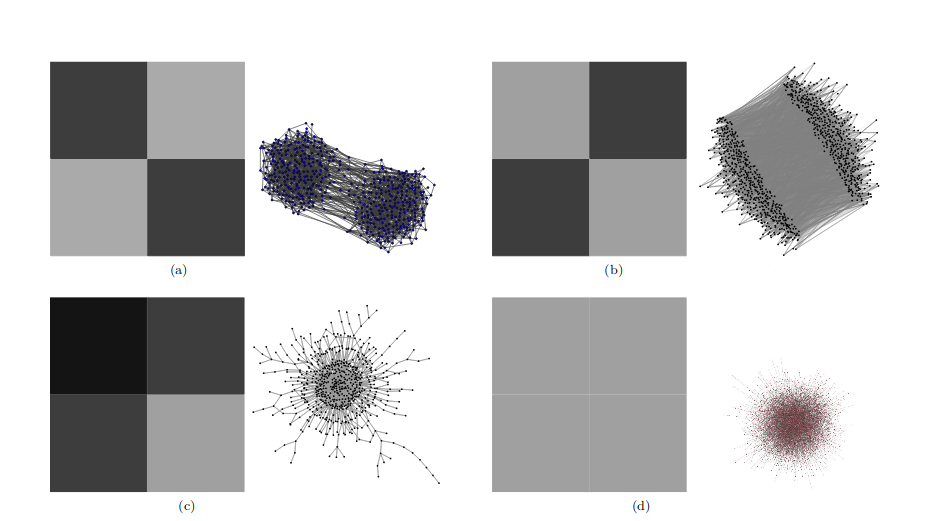
\includegraphics[width=0.5\textwidth]{Figures/structures.png}
	\caption{Stochastic Block model for different networks structures. (a) assortative. (b) dissortative. (c) core-periphery. (d) Erdos Renyi random graph.}
	\label{fig:SBM}
\end{figure}

A common definition of a community is that it is densely connected subgraph \cite{userguide}. We can find these subgraphs by optimizing an objective function, such as modularity function. It measures the difference in the number of edges between the given network and the network with the same number of nodes but randomly connected. In this approach, we try to maximize the density of connections inside a group by focusing more on assortative\footnote{Networks where nodes tend to connect with other nodes of a similar degree. Edges are more likely inside blocks than out of them.} group structures. 

Another type of networks is the bipartite network that has two disjoint sets of nodes. The edges exist only between nodes from different sets. Networks of this class can appear in real-world data, such as users-movies preference, collaboration network for scientists and papers, etc. Application of density-based approach requires to first project bipartite network to one of its partitions and then find communities in that projection. With this, some information is lost. On the other hand, the method that is directly applicable to bipartite networks is Stochastic Block model, from which the models considered in this paper are derived. \\

Stochastic block model (SBM) is based on connection probabilities between nodes. It is a generative model which includes existence of communities. Parameters that describe SBM for network G with N nodes are:

\begin{itemize}
	\item k: number of groups
	\item group assignment vector, g: $g_i \in\{1,2..k\}$, gives the group index of node $i$.
	\item SBM matrix, $p_{k \times k}$, whose elements $p_{ij}$ are the probabilities that edges between groups $g_i$ and $g_j$ exist.
\end{itemize}

Note that nodes within one group have the same connection probabilities.

SBM can generate and describe different types of network structures. Figure \ref{fig:SBM} \cite{userguide} shows how the model matrix corresponds to resulting networks with two communities. First, for the assortative network (\ref{fig:SBM} a), diagonal elements of the matrix have higher probabilities. This indicates dense connections inside the group, just like in classic community structures. In disassortative structure, (\ref{fig:SBM} b), more connections exist between two partitions than inside them, i.e. off-diagonal elements have higher probabilities. Bipartite networks can be represented like this. 

Figure (\ref{fig:SBM} c) shows how the model represents core-periphery networks. Nodes of one block (core) are well connected with itself and with other partition (periphery). From the last case, we can note that SBM with one group is the Erdos Renyi random graph (\ref{fig:SBM} d) because all probabilities inside and between groups are equal.

The benefit of this model is that we can generate many networks with similar group structure. The model can fit real data, which results in finding network communities. For the given network $G$ and number of groups $k$, the best nodes partition $g$ is found by maximizing the likelihood function. Beside inferring communities, SBM has application in prediction of missing links. This simply formulated model has many variants, motivated by specific properties of real data. For example, for networks which are degree heterogeneous, there is degree corrected SBM. In some social networks, users can belong to more than one group, and this can be modelled with mixed membership SBM. Other extensions include application to bipartite, weighted network, hierarchical model, etc. Also, several algorithms for optimization of likelihood function are proposed. The overview of these versions and methods are given in \cite{comparison}. In this paper, we will focus on Single and Mixed Membership SBM applied on bipartite networks.  




\section{The measures of networks}

The complex system can be represented by complex network $G=(V, E)$, where the elements of system (atoms, proteins, people) map to set of $N$ nodes $V=\{1, 2, ...,N\}$. The interactions between elements map to $L$ links between nodes, $E = \{ e_1, e_2... e_L\}$. The \textbf{adjacency matrix} ${A} = N \times N$ has value $1$ if there is connection between two nodes, otherwise it is $0$ \cite{boccaletti2006}. 

\subsection{degree distribution}

%The degree of a node is the number of links that involve that node, which is the cardinality of i’s neighborhood. Thus, a node i’s degree in a network g, denoted d i (g), is d i (g) = #fj : g ji = 1g = #N i (g): In the case of a directed network, the above calculation would be the in-degree. The out-degree of node i is the corresponding calculation #fj : g ij = 1g. These coincide in the case of an undirected network. The density of a network keeps track of the relative fraction of links that are present, and is simply the average degree divided by n 1.

The network properties directly depend on the connectivity between nodes. In the case of regular networks, such as grids, each node has an equal number of first neighbours. In the general case, the networks have a more complicated structure. Thus the important measure is network \textbf{degree} $k$. The degree of node $i$ gives the number of nodes attached to node $i$, $k_i = \sum_j A_{ij}$. The \textbf{degree distribution} $P(k)$ is probability that randomly chosen node has degree $k$. It can be calculated as fraction of $k$ degree nodes $N_k$, $p(k) = N_k/N$. The degree distribution in random network, where all nodes have the same connecting probability, follows Poisson distribution $P(k)= \frac{(Np)^ke^{-Np}}{k!}$, where $k$ is the mean degree distribution. In real networks degree distribution follows a power law. Therefore, real networks have a scale-free structure with the emergence of the hubs \cite{newman2010}.

\subsection{assortativity}
The \textbf{degree-degree correlations} in the network are measured by \textbf{assortativity}. If correlations are positive, networks are assortative; there is a tendency that connections exist between similar degree nodes. The negative correlations indicate that large degree nodes have preference to connect nodes with small degree; dissasortative networks. The average first neighbor degree $k_{nn}$ can be calculated as $k_{nn} = \sum_{k^{'}}k^{'}P(k^{'}|{k})$. The $P$ is conditional probability that an edge of degree $k$ points to node with degree $k$. The norm is $\sum_{k^{'}}P(k^{'}|k)=1$, and detailed balance conditions \cite{boccaletti2006},  $kP(k^{'}|k)P(k) = k^{'}P(k|k^{'})P(k^{'})$ \cite{boccaletti2006}. If the node degrees are uncorrelated, $k_{nn}$ does not depend on the degree, otherwise increasing/decreasing function indicates on positive/negative correlations in the network.

The Newman defined the assortativity index $r$ in slightly different way:
$r = \sum_{kl}kl(e_{kl} - q_lq_k) / \sigma_q^2$, where $e_{kl}$ is the probability that randomly selected link connect nodes with degrees $k$ and $l$, $q_k$ is probability that randomly choosen node is connected to node $k$ and equals $q_k = kp_k / \langle k \rangle$, while $\sigma_q$ is varience of the distribution $q_k$. 

\subsection{clustering coefficient}
The \textbf{clustering coefficient} is a measure describing the neighbourhood's structure. In networks exist tendency to form triangles or clusters. This is common in friendship networks where two friends of one person have a high probability of being friends. The clustering can be measured by computing the number of links between neighbours of one node, $c_i=2e_i/(k_i(k_i-1))$. Averaging it over all network nodes, we can calculate the mean clustering coefficient. It ranges from  $\langle c \rangle = 0$ where connections between neighbouring nodes do not exist, network has the structure of three. On the other hand, $\langle c \rangle = 1$ indicates a fully connected network. 

\subsection{real-world networks}
Real-world networks share similar properties. The mean distance between nodes is smaller than the number of nodes in the network $l << N$, called small-world phenomena. This cause the fast spread of information or even diseases in the complex systems. In small-world networks number of vertices grow exponentially with distance; thus $l$ increase as $log(n)$ or slower. Logarithmic scaling can be proved from various network models; also, it is observed in real-world complex systems. The clustering coefficient in real-world networks is usually high. Real-world networks have one important feature; power-law degree distribution; such networks are called scale-free networks.

\subsection{D-measure}

Between two nodes in the network, we can define different paths, but the most important one are the shortest paths, $d_{ij}$. Diameter defines the largest shortest path found in the network. For each node $i$ we can define the distribution of the shortest paths between node $i$ and all others nodes in the network, $P_{i}=\{p_{i}(j)\}$, where $p_{i}(j)$ is percent of nodes at distance $j$ from node $i$. The connectivity patterns can efficiently describe difference between two networks.    
To specify how much $G$ and $G^{'}$ are similar we use D-measure \cite{tiago2}

\begin{equation} 
\label{eq:dmeasure}
D(G,G') = \omega \left| \sqrt{\frac{J(P_1,..P_N)}{log(d)}}-\sqrt{\frac{J(P_1^{'},..P_N^{'})}{log(d^{'})}} \right| \nonumber +  (1-\omega) \sqrt{\frac{J(\mu_{G},\mu_{G^{'}})}{log2}}.
\end{equation}

D-measure calculates Jensen-Shannon divergence between $N$ shortest path distributions, $J(P_1,.., P_N)) = \sum_{i,j}p_i(j)log(\frac{p_i(j)}{\mu_j})$, where  $\mu_j = (\sum_{i=1}^N p_i(j))/N$ is mean shortest path distribution. The first term in equation \ref{eq:dmeasure} compares local differences between two networks, and Jensen-Shannon divergence between $N$ shortest path distributions $J(P_{1},...,P_{N})$ is normed with network diameter $d$. The second part determines global differences, computing  ${J(\mu_{G},\mu_{G^{'}})}$ between mean shortest path distributions. We consider equally important local and global properties of the networks, and parameter $\omega$ is set to $0.5$. The D-measure ranges from $0$ to $1$. The lower D-measure is, networks are more similar and for D-measure $D = 0$, structures are isomorphic.






